\documentclass[a4paper,11pt,titlepage,uplatex]{jsarticle}

% プリアンブルを外部ファイル化しておきました。中身はmacro.texで確認できます。

\usepackage[dvipdfmx]{graphicx,xcolor}% ドライバ指定
\usepackage[top=30truemm,bottom=30truemm,left=25truemm,right=25truemm]{geometry} % 余白設定

% 画像
\usepackage{here, subfig}
\usepackage{docmute} % ファイル分割用
\usepackage[cc]{titlepic}

% 数式関連
\usepackage{amsmath,amsfonts,amssymb,mathtools,amsthm}
\usepackage{bm} % ボールド体のベクトルを出力するときには\vb{a}ではなく\bm{a}としてください。\bmの方が綺麗に出力できる。
\usepackage{empheq} % 連立方程式をきれいに書いてくれる
\usepackage{physics} % 微分記号とか
\usepackage[separate-uncertainty]{siunitx} % SIUNITX

% 数式、図、表番号の変更
\makeatletter
\@addtoreset{equation}{section} % 章ごとに番号をリセット
\@addtoreset{figure}{section}
\@addtoreset{table}{section}
\def\theequation{\thesection.\arabic{equation}} % 章.何番目 と変更
\def\thefigure{\thesection.\arabic{figure}}
\def\thetable{\thesection.\arabic{table}}
\makeatother

% -------------------
% 定理環境付近
\usepackage{tcolorbox} % 色付きの囲み
\tcbuselibrary{breakable, skins, theorems}
\usepackage{ascmac} % 囲み \begin{itembox}ができる。

% ----------

\usepackage{enumitem} % enumium環境いじるために必要
\renewcommand{\labelenumi}{\theenumi.}
\renewcommand{\theenumi}{\Alph{enumi}}

% ------------ url関係
\usepackage{url}
\usepackage[dvipdfmx]{hyperref}
\hypersetup{
	 colorlinks=true,
	 citecolor=blue,
	 linkcolor=black,
	 urlcolor=blue
}
\usepackage{pxjahyper}
% ---------

% 表関連のパッケージ
\usepackage{booktabs}
\usepackage{multirow}
\usepackage{longtable}
\usepackage{arydshln}% 表で破線を使うため
\usepackage{multicol}
% longtableをusepackageする場合は順番が重要らしいです。longtableとarydshlnの順番逆にしたらエラーはく(コンパイルはできるが…)

\renewcommand{\labelitemii}{・}

\usepackage[greek, japanese]{babel}
\usepackage{teubner}	% 古代(古典)ギリシア語表記指定



% 大槻使用
\usepackage{color}
\newcommand{\red}[1]{\textcolor{red}{#1}}
\newcommand{\blue}[1]{\textcolor{blue}{#1}}
\usepackage{ulem}

% 能崎使用
%背景
\usepackage{wallpaper}

\begin{document}

% \tableofcontents % 目次を作成
\newpage
\section{電装概要}
電装タワー上段からGPS基板、開放基板、ミッション基板の3つの基板を搭載した。
GPS基板と開放基板はマイコンにSTM32-F446RET6を、ミッション基板はESP32を搭載した。
記憶素子はSPI flashであるS25FL127を搭載した。基板動作用電源としてCR-123Aを4個、動翼用電源としてLi-Feバッテリーを搭載した。
電源回りの配線を図\ref{fig:battrey}に示す。また電装タワー全体の配線の模式図を図\ref{fig:tower_all}に示す。
さらに実際の電装タワーの外観を図\ref{fig:avi_tower}に示す。

\begin{figure}[H]
	\centering
	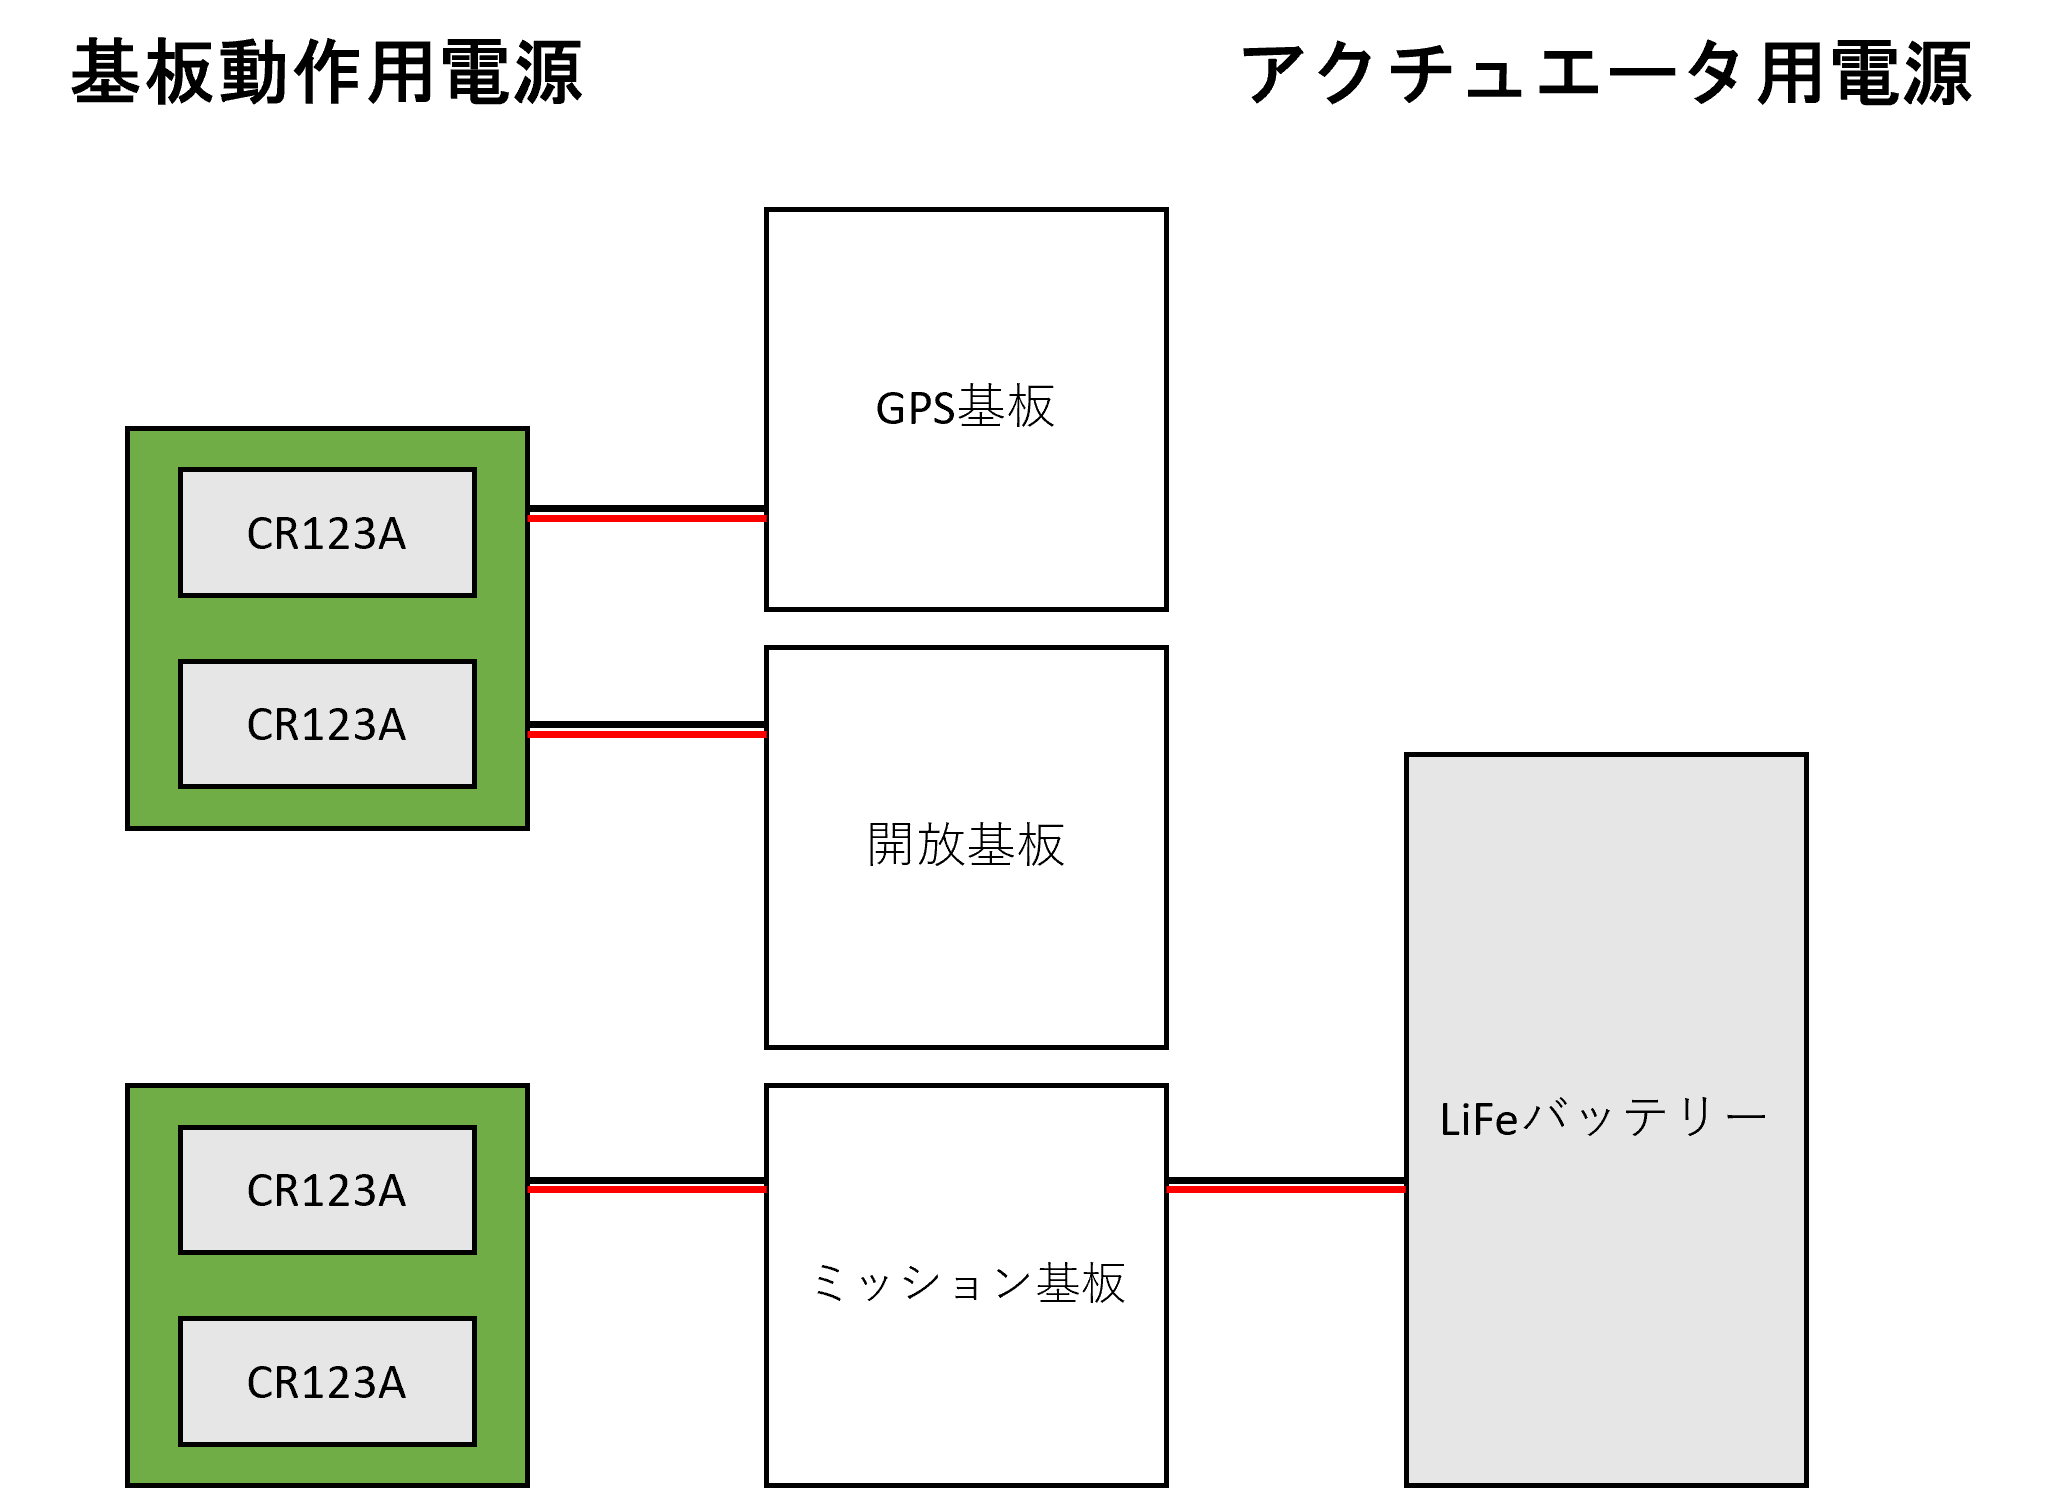
\includegraphics[width=0.8\linewidth]{pic_avi/battery.png}
	\caption{電源供給}
	\label{fig:battrey}
\end{figure}

\begin{figure}[H]
	\centering
	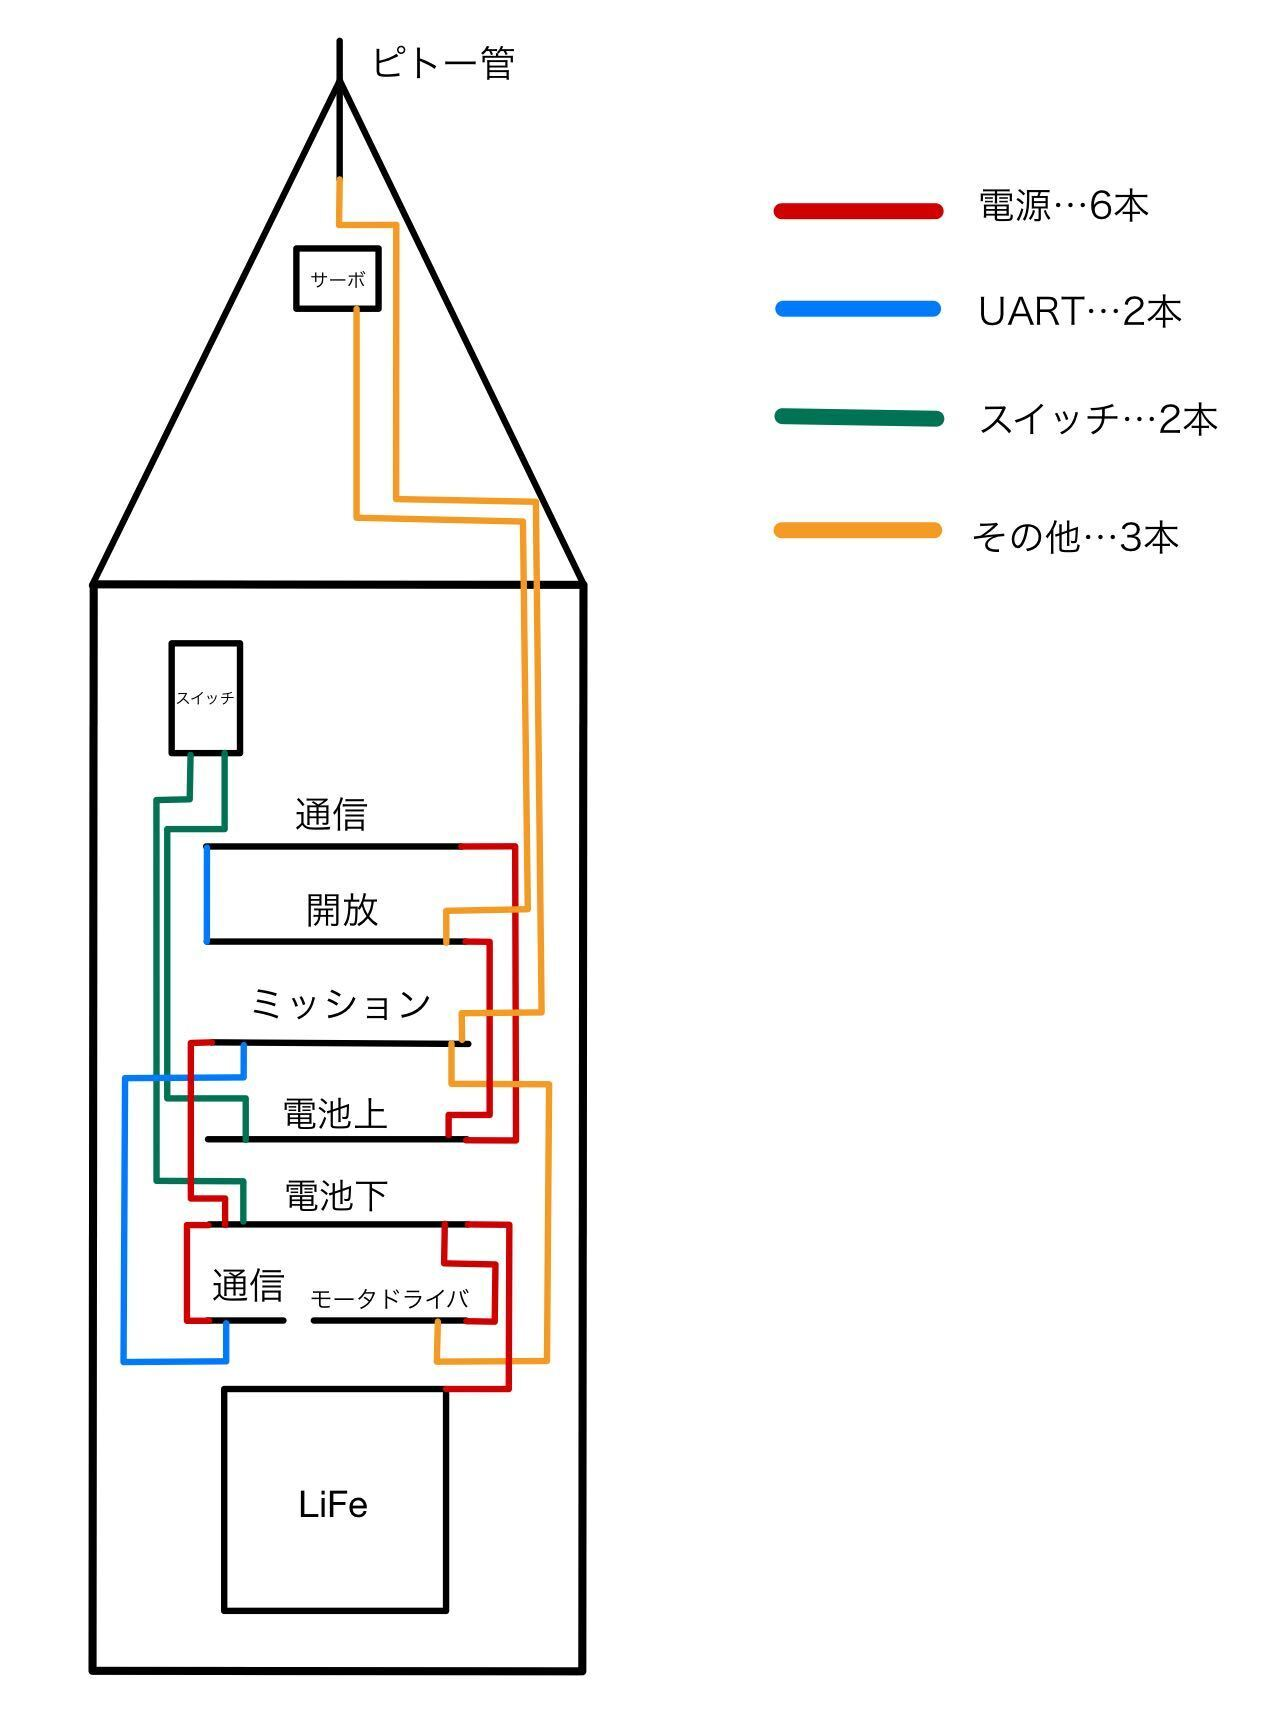
\includegraphics[width=0.5\linewidth]{pic_avi/avi_tower_line.jpg}
	\caption{電装タワー全体の配線}
	\label{fig:tower_all}
\end{figure}

\begin{figure}[H]
	\centering
	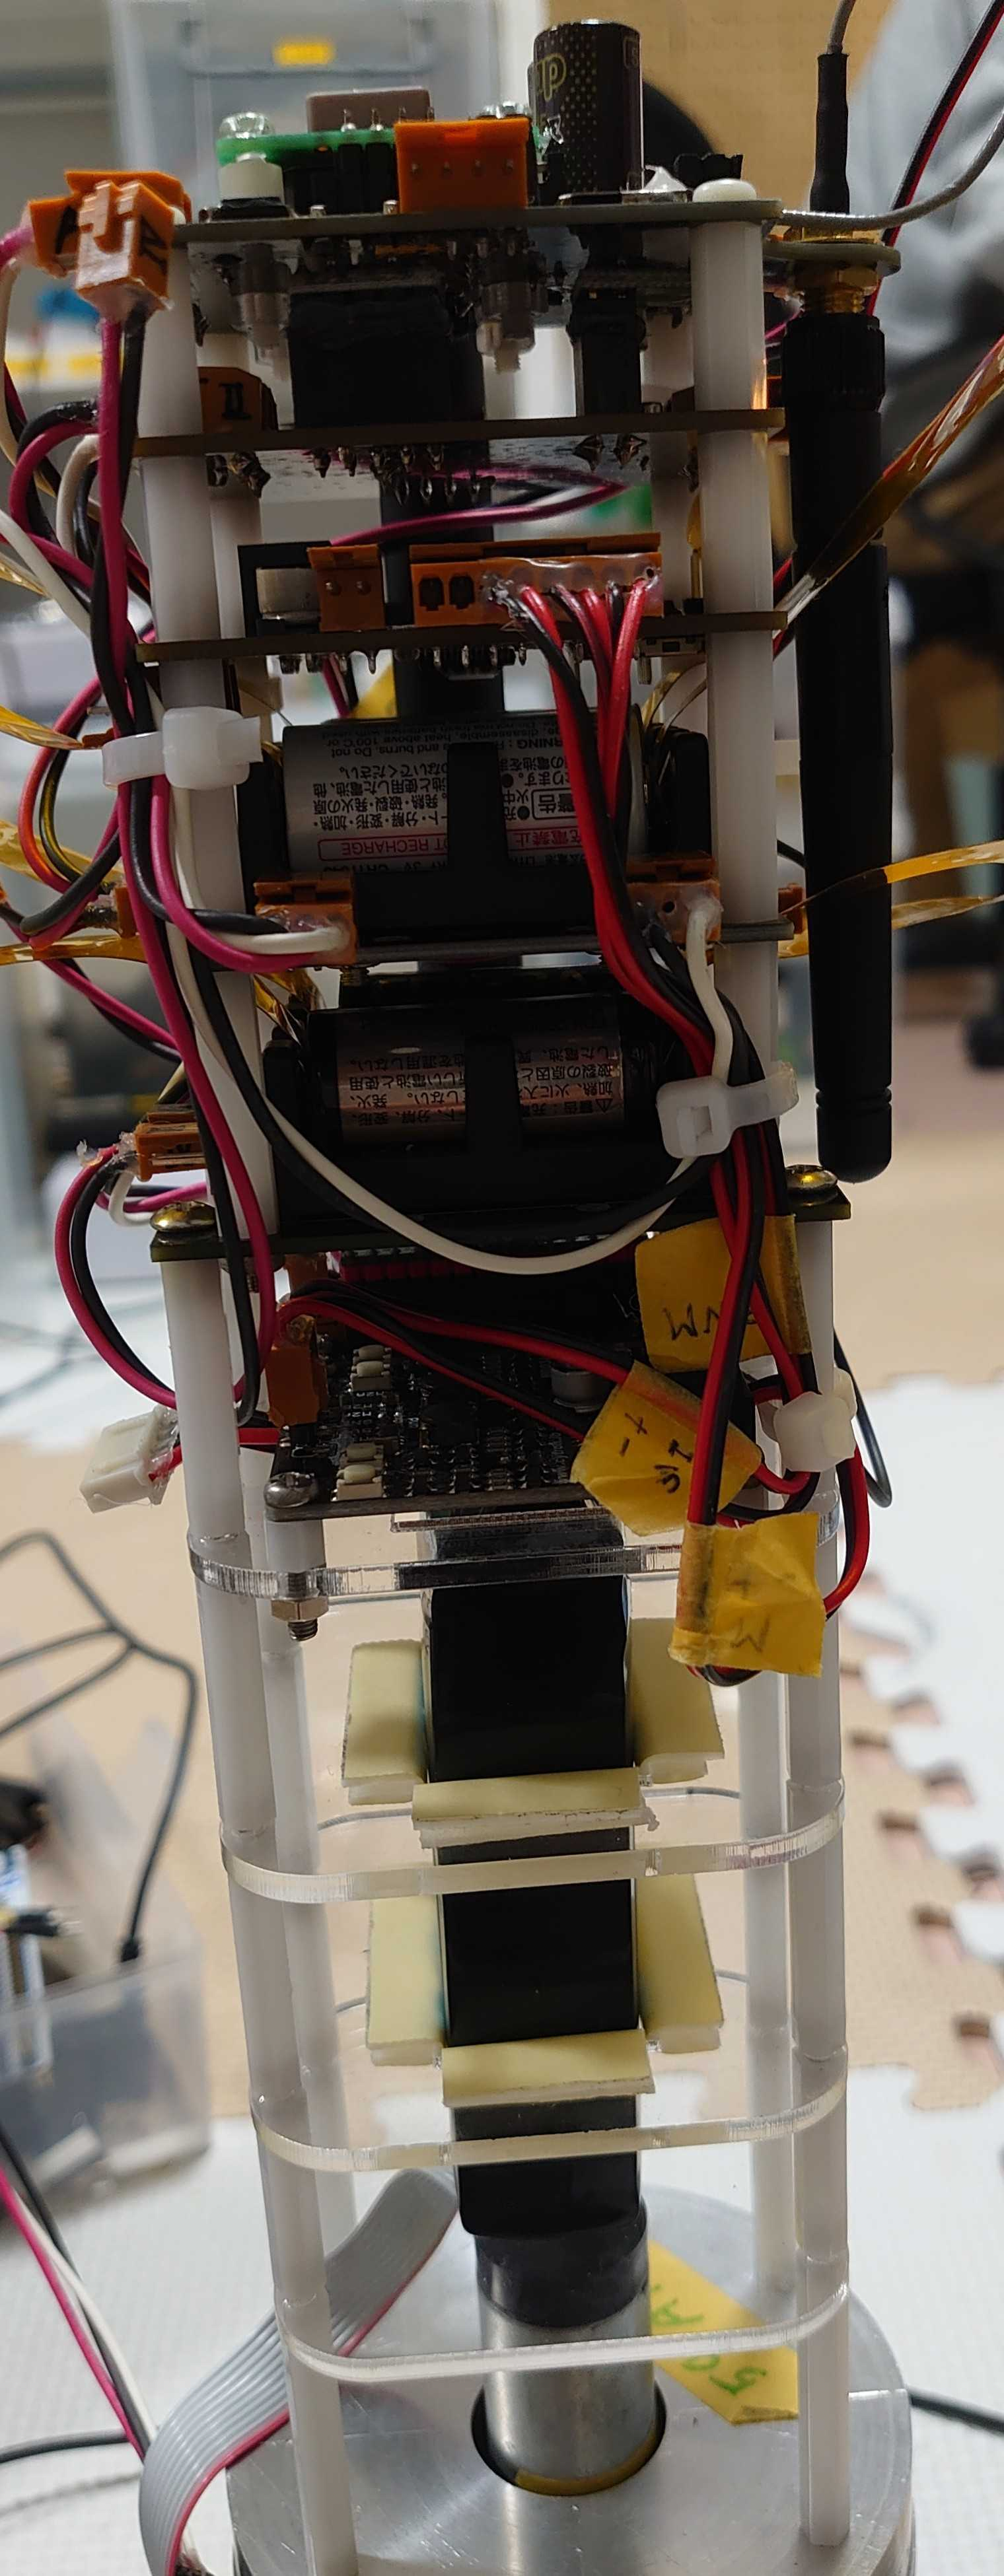
\includegraphics[width=0.25\linewidth]{pic_avi/avi_tower.JPG}
	\caption{電装タワー外観}
	\label{fig:avi_tower}
\end{figure}

\subsection{GPS基板}
\begin{itemize}
	\item 役割
	      \begin{itemize}
		      \item GPS位置座標の取得、記録
		      \item 無線通信による開放基板へのコマンド操作
	      \end{itemize}

	\item 搭載モジュールの詳細(表\ref{tab:com_detail})
	      \begin{table}[H]
		      \centering
		      \caption{通信基板のセンサ等詳細}
		      \begin{tabular}{cccc} \toprule
			      センサ等種類 & 型番           & サンプリングレート (\si{Hz}) & 測定範囲 \\ \midrule
			      GPS    & AE-GYSFDMAXB & 10                  & -    \\
			      無線     & TWE-Lite-RED & -                   & -    \\
			      \bottomrule
		      \end{tabular}
		      \label{tab:com_detail}
	      \end{table}
\end{itemize}

\subsection{開放基板}
\begin{itemize}
	\item 役割
	      \begin{itemize}
		      \item 減速機構の開放動作
		      \item \SI{1}{kHz}での加速度、角速度のロギング
		      \item \SI{50}{Hz}での気圧のロギング
	      \end{itemize}

	\item 搭載モジュールの詳細(表\ref{tab:para_detail})
	      \begin{table}[H]
		      \centering
		      \caption{開放基板のセンサ等詳細}
		      \begin{tabular}{cccc} \toprule
			      センサ等種類 & 型番       & サンプリングレート (\si{Hz}) & 測定範囲                          \\ \midrule
			      加速度    & MPU-9250 & 1000                & \SI{+-16}{G}                  \\
			      角速度    & MPU-9250 & 1000                & \SI{+-2000}{deg/sec}          \\
			      気圧     & LPS-22HB & 50                  & \SI{260}{hPa}から\SI{1260}{hPa} \\
			      \bottomrule
		      \end{tabular}
		      \label{tab:para_detail}
	      \end{table}

	\item 離床検知条件
	      \begin{enumerate}
		      \item 各軸それぞれの加速度センサの直近の値20回分(=0.02秒間分)の平均値を$\bar{a}_x,\,\bar{a}_y,\,\bar{a}_z$とする。このとき、
		            \begin{equation}
			            \sqrt{{\bar{a}_x}^2 + {\bar{a}_y}^2 + {\bar{a}_z}^2} > \SI{2}{G}
		            \end{equation}
		            を50回連続で満たしたとき
		      \item 気圧センサの直近の値5回分(=0.1秒間分)の平均を取り、この値が前回の値より \SI{0.1}{hPa}以上低い状態が1秒間連続したとき
	      \end{enumerate}
	      上記のうちいずれかが1つを満たしたとき、その1秒前を離床時刻とする。

	\item 頂点検知条件
	      \begin{enumerate}
		      \item 離床検知から3秒以上経過していること
		      \item 離床から10.65秒後
		      \item 0.1秒ごとに気圧センサの値の5回分の平均値を取り、この平均値が前回の平均値より高い状態が1秒間連続すること
	      \end{enumerate}
	      上記のうちAを満たし、かつB、Cのうち1つの条件を満たしたときに減速機構を開放する。
\end{itemize}


\subsection{ミッション基板}
\begin{itemize}
	\item 役割
	      \begin{itemize}
		      \item 動翼を用いたロール制御
		      \item \SI{500}{Hz}での加速度、角速度、対気速度のロギング
	      \end{itemize}

	\item 搭載モジュールの詳細(表\ref{tab:mission_detail})
	      \begin{table}[H]
		      \centering
		      \caption{通信基板のセンサ等詳細}
		      \begin{tabular}{cccc} \toprule
			      センサ等種類 & 型番              & サンプリングレート (\si{Hz}) & 測定範囲                 \\ \midrule
			      加速度    & MPU-9250        & 500                 & \SI{+-16}{G}         \\
			      角速度    & MPU-9250        & 500                 & \SI{+-2000}{deg/sec} \\
			      差圧計    & HSCDRRN100MDSA3 & 500                 & \SI{+-100}{mbar}     \\
			      無線     & TWE-Lite-RED    & -                   & -                    \\
			      \bottomrule
		      \end{tabular}
		      \label{tab:mission_detail}
	      \end{table}
\end{itemize}

\subsection{データ回収}
\subsubsection{GPS基板}
離床から地上に落下する数秒前まではGPSのデータを回収に成功した。
しかし、地上に落下する少し手前で通信が途絶した。開傘の衝撃によってGPSのセンサー部分が破損し、受信ができなくなったことが主な原因だと考えられる。

\subsubsection{開放基板}
\SI{1000}{Hz}で加速度・角速度、\SI{50}{Hz}で気圧データの回収に成功した。

\subsubsection{ミッション基板}
\SI{500}{Hz}で加速度・角速度、対気速度データの回収に成功した。

\subsection{過去機体からの改良点・新技術}
\subsubsection{動翼を用いたロール制御}

\subsubsection{ピトー管}

\subsubsection{スイッチ機構}
\label{switch}
CREATEでは毎回の打ち上げで電池の持ちがネックとなっていた。
そこで今回はスイッチ機構を搭載した。
図\ref{avi_switch_out}のつまみ付きジャンパピンを抜くと、電源が接続し、つけたままだと電源が遮断される仕組みとなっている。
内側は図\ref{avi_switch_in}のように3Dプリンターの治具と基板のモジュールでできており、配線がILGコネクタ―につながることで、電池基板とつないでいる。
1日目、9:30から16:00までの6時間半のほとんどの時間を電源を遮断していたが、開放通信基板の電圧は\SI{6.5}{V}から\SI{5.98}{V}に降下していた。
これはP型FETの回路内の抵抗の消費電力とサーボモータの待機電力が大きかったことが挙がられる。
次機体以降は外部給電を用いて電池の持ち時間に困らないシステムを構築したい。

\begin{figure}[H]
	\begin{tabular}{cc}
		\begin{minipage}[t]{0.45\hsize}
			\centering
			\includegraphics[scale = 0.05]{pic_avi/switch2_out.jpg}
			\caption{スイッチ機構(内側)}\label{avi_switch_in}
		\end{minipage} &
		\begin{minipage}[t]{0.45\hsize}
			\centering
			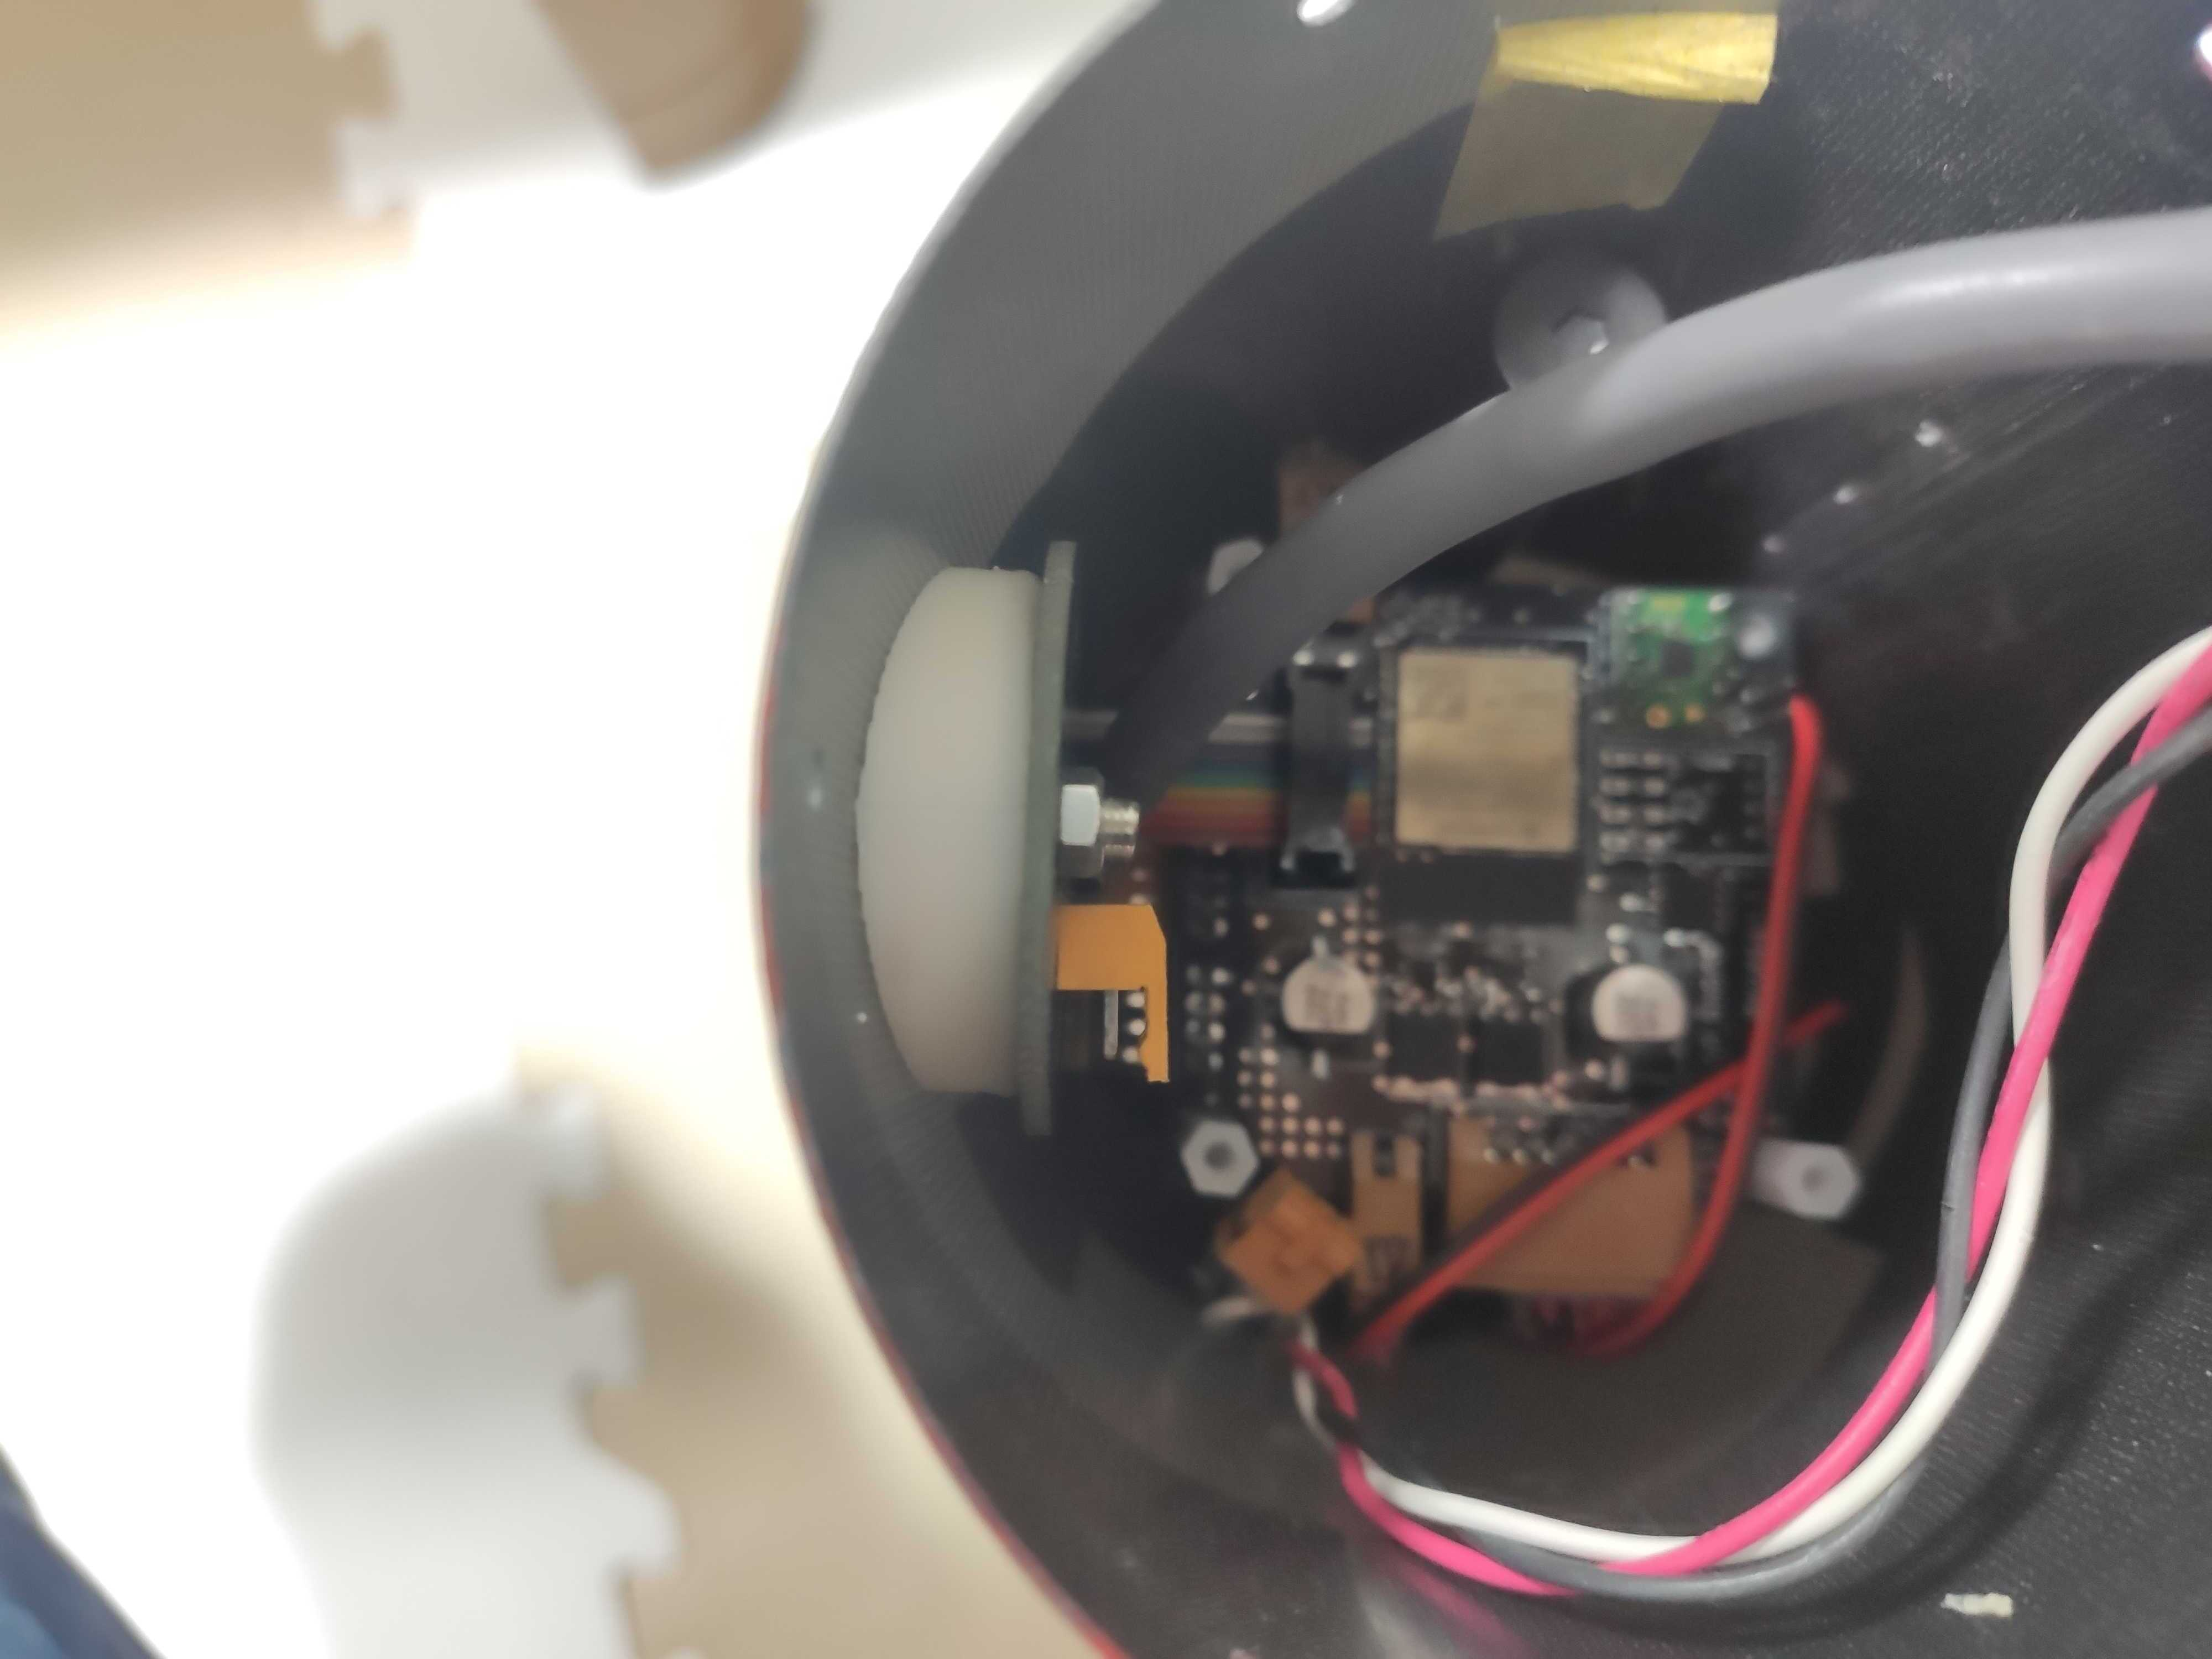
\includegraphics[scale = 0.05]{pic_avi/switch_in.jpg}
			\caption{スイッチ機構(外側)}\label{avi_switch_out}
		\end{minipage}
	\end{tabular}
\end{figure}



\subsubsection{GPSデータプロットソフト}
地上局で受信したGPS信号を短期間で処理し、GoogleEarthに経路を表示するソフトを開発した。このソフトによって、打ち上げ10分後には部員にプロットデータを配布できた。実際のGoogleEarthの経路を図\ref{fig:GPS_plot}に示す。
\begin{figure}[H]
	\centering
	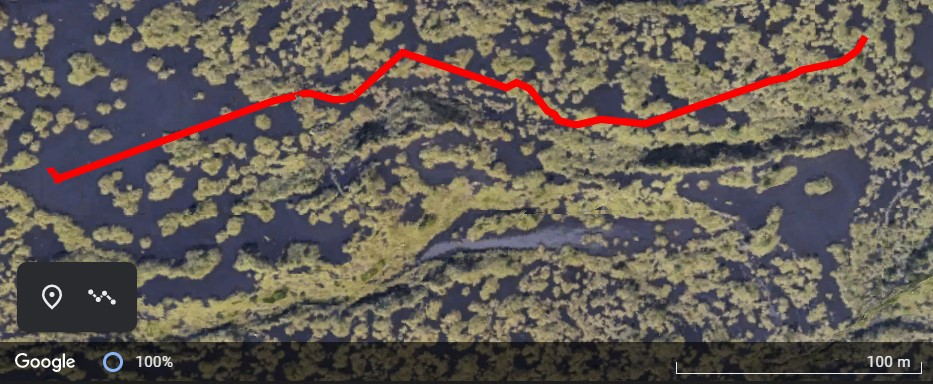
\includegraphics[width=0.8\linewidth]{pic_avi/GPS_plot.jpg}
	\caption{ソフトでのプロットの様子}
	\label{fig:GPS_plot}
\end{figure}



\subsection{離床検知}
打上動画及び各基板の機軸方向加速度データから、エンジンが振動燃焼を起こしていた可能性は大きいと考えられる。
開放基板の$z$軸方向(機軸方向、前方正)加速度の離床直前から燃焼終了後までの推移を図\ref{fig:az_data}に示す。
開放基板は直近20回分の加速度の平均値を算出し、\SI{50}{Hz}で加速度による離床検知を行った。
直近の加速度の平均値が1秒間連続して\SI{2}{G}を超えていれば離床と判断するため、振動燃焼による加速度のばらつきを吸収し、加速度で離床検知ができた。
\begin{figure}[H]
	\centering
	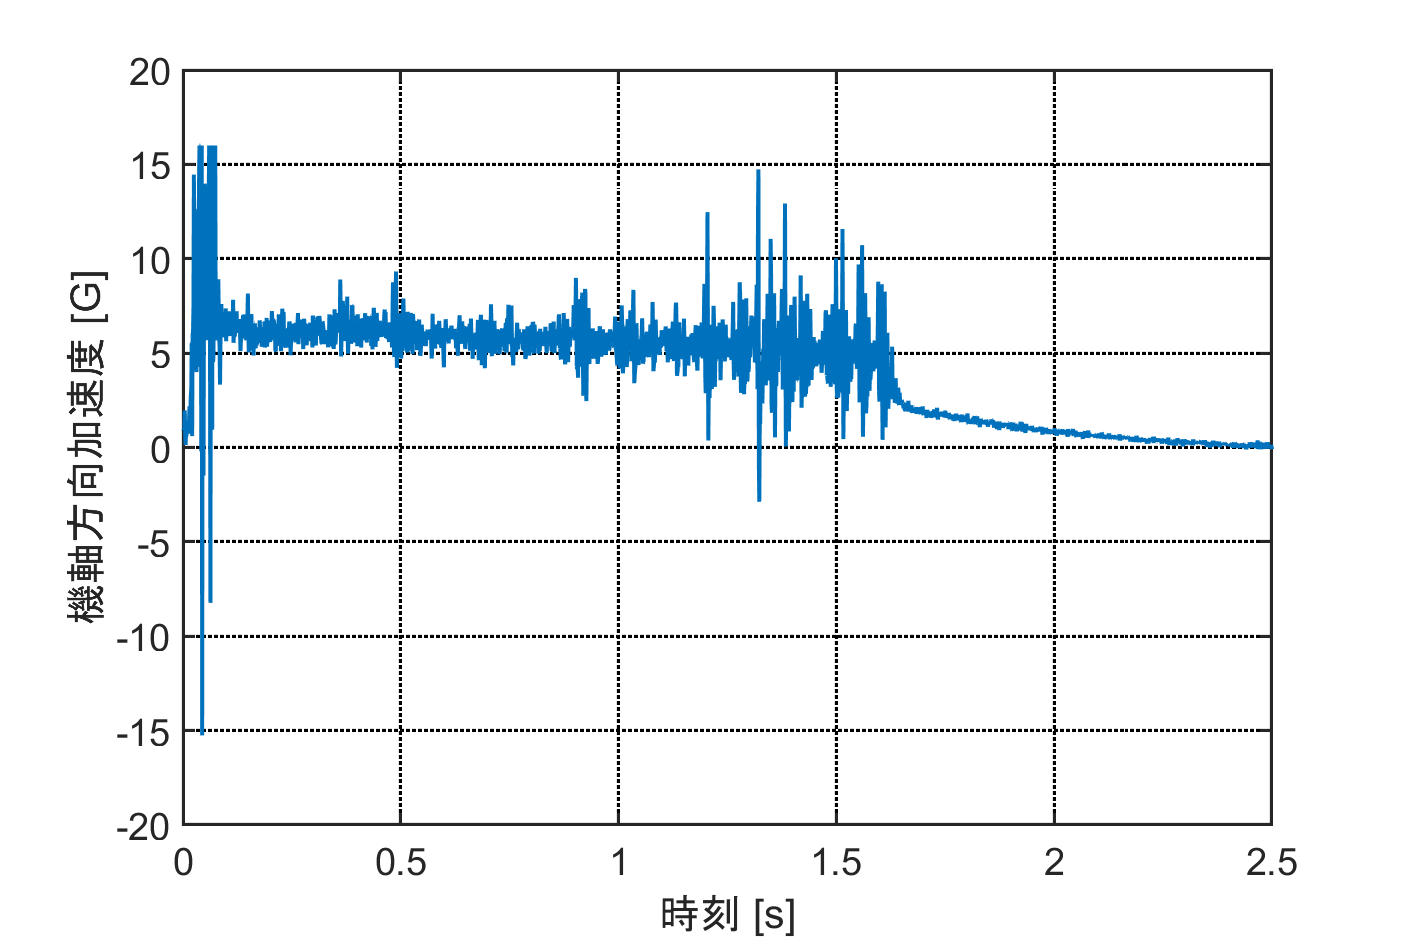
\includegraphics[width=0.8\linewidth]{pic_avi/59_6axis.png}
	\caption{機軸方向の加速度の時間推移(開放基板)}
	\label{fig:az_data}
\end{figure}

\subsection{ランチクリア速度}
まず、点火点から撮影した映像を元に算出したところ約\red{\SI{23.6}{m/s}}だった。
一方、基板のデータからも算出した。加速度を積分し速度を、もう一度積分し距離を求めた。
その結果速度は約\SI{23.19}{m/s}だった。


\subsection{到達高度}
図\ref{fig:height_data}は開放基板の気圧センサのデータから求めた離床からの時刻と高度の関係である。
最高到達高度は約\SI{353}{m}である。算出に使用する気温は、大島のアメダスの打上時刻付近の気温と、アメダス設置点と射点の高度差から推測した気温\SI{16.82}{\degreeCelsius}を使用した。
\begin{figure}[H]
	\centering
	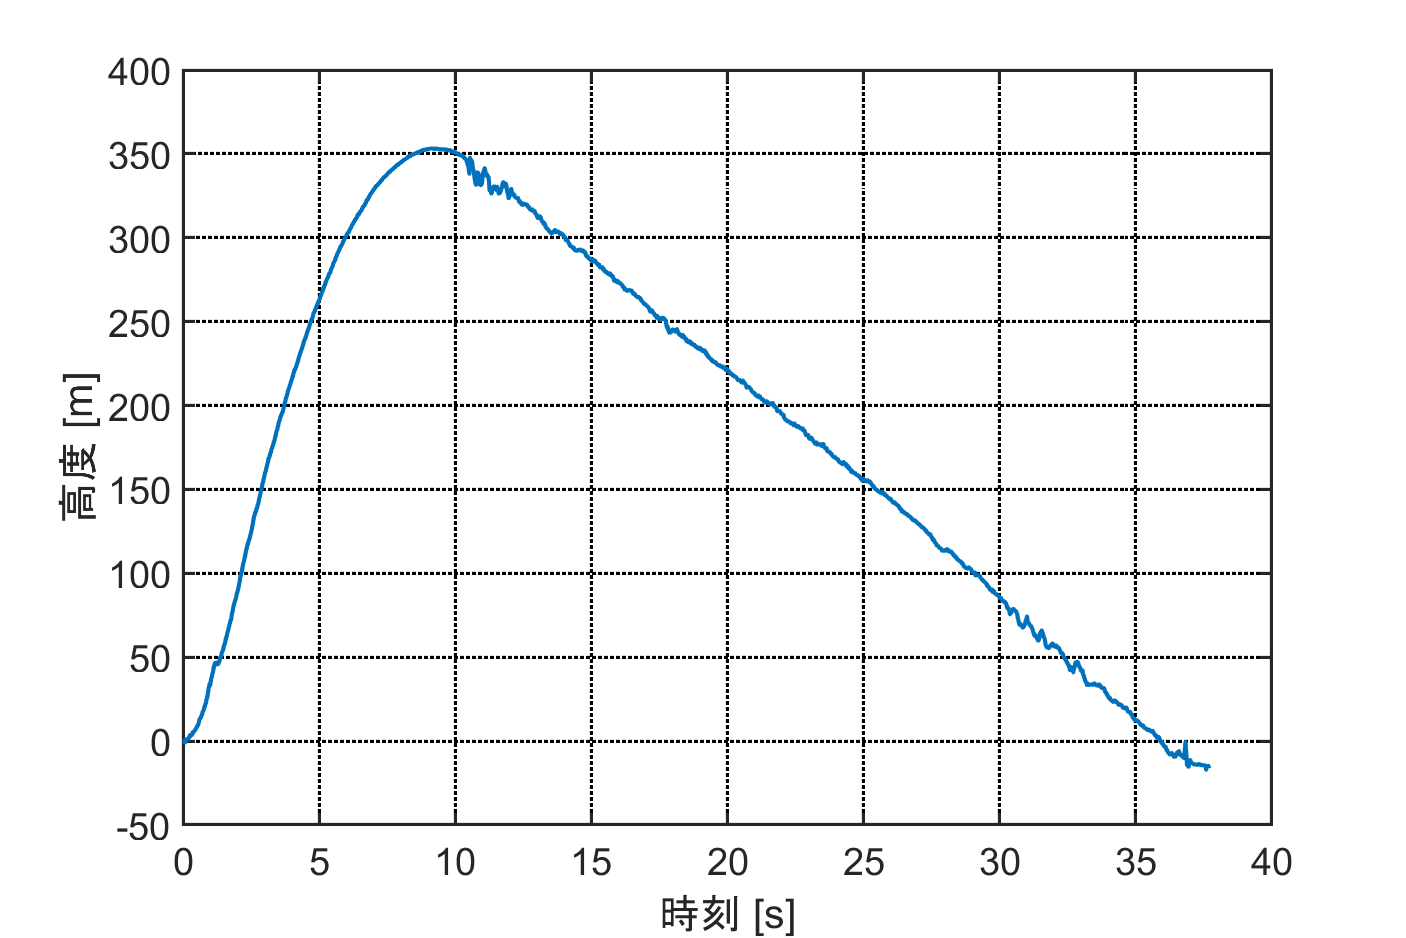
\includegraphics[width=0.8\linewidth]{pic_avi/height_data.png}
	\caption{離床からの時刻と高度の関係}
	\label{fig:height_data}
\end{figure}


\subsection{減速機構開放}
離床から10.2秒後に減速機構を開放した。タイマー条件ではなく、冗長系の気圧条件で頂点検知をして開放していたことがログから確認された。
実際の最高到達高度が\SI{353}{m}であったのに対し、予想最高到達高度が\SI{383}{m}だったため、頂点到達時刻が早くなったことが原因として考えられる。またデータからは頂点到達後約1.1秒後に減速機構に指令がなされていた。
頂点到達後1秒以内に減速機構に指令を出す想定でいたため、約0.1秒程度遅い展開となった。

\subsection{落下位置推定}
飛行中のGPSの電波を受信できた。
しかし、今回GPS最終受信地点は実際の落下地点と比較して直線距離で約\SI{60}{m}ずれてしまった。(図\ref{fig:GPS_data})
大きなずれが生じてしまった理由として、開傘衝撃でセンサーが破損し、落下の途中までしかGPSデータをダウンリンクができなかったことだと考える。
今回GPSのデータが受信できていると確認できたため、指差しによる落下位置推定を行わなかった。しかし、ずれが大きかったことから、指差しによる落下位置推定を行うべきであった。
次回以降の打ち上げでは確実に行えるように準備したい。

\begin{figure}[H]
	\centering
	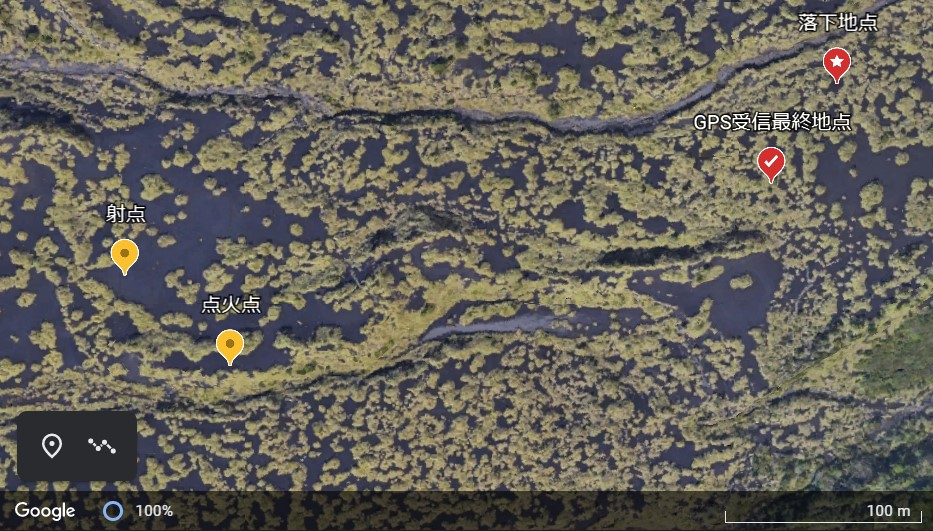
\includegraphics[width=0.8\linewidth]{pic_avi/GPS_data.jpg}
	\caption{GPS最終受信地点と実際の落下地点}
	\label{fig:GPS_data}
\end{figure}

\subsection{動翼を用いたロール制御}
\subsubsection{概要}
エンジン燃焼終了後からパラシュート開傘までの間、機体のロール角を一定値に保つ制御を行った。エンコーダ付きDCモータを用いて動翼の角度を制御し、空力によって発生するロールモーメントを用いて制御した。
\subsubsection{ハードウェア構成}
動翼角度を制御するために、MAXON社製のエンコーダ付きギアモータを使用した。モータはA-max22(製品番号110158)を使用した。
良好な制御特性を得るために慣性モーメントの小さいコアレスモータを用いることとし、比較的価格が安いA-maxシリーズを採用した。
ギアヘッドは、減速比29.16のプラネタリギアを用いた。十分なトルクと動翼回転速度を両立する減速比を採用した。低バックラッシ品の採用は、価格を考慮し断念した。
エンコーダは、512パルス/回転で2相のインクリメンタルエンコーダを用いた。動翼角度の分解能は、4逓倍を用いて$360/512/4/29.16\simeq 0.006\,[\mathrm{deg}]$である。
使用したセンサの詳細は\red{ミッション基板のセンサ等詳細}に記述した。動翼機構の詳細は\red{(構造班のところ)}に記述した。
\subsubsection{制御則}
図\ref{fig:ブロック線図}に対気速度がある値$v$のときの、制御器と制御対象をモデル化したブロック線図を示す。
\begin{figure}[H]
	\centering
	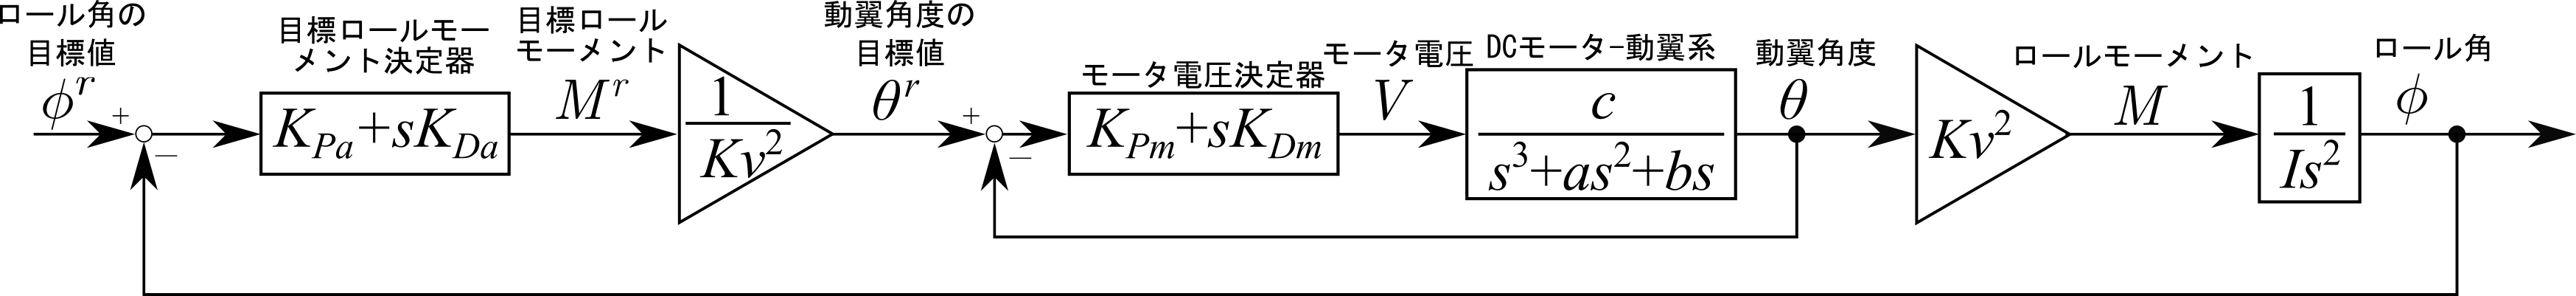
\includegraphics[width=0.95\linewidth]{pic_avi/block_diagram.png}
	\caption{ブロック線図}
	\label{fig:ブロック線図}
\end{figure}
対気速度はピトー管により計測される。制御対象であるロール角とロールモーメントの関係は、
\begin{equation}
	I\ddot\phi=M
\end{equation}
によりモデル化する。ただし$I$はロール方向の慣性モーメント、$\phi$はロール角、$M$は動翼が発生させるロールモーメントである。
動翼が発生させるロールモーメントの目標値$M^r$は、目標ロールモーメント決定器がPD制御を用いて決定する。$K_{Pa}$がPゲイン、$K_{Da}$がDゲインである。
エンコーダ付きギアモータの出力を傘歯車を介して伝えることで、2枚の動翼を駆動する。これらの機構を合わせてモータ-動翼系と呼称する。モータ-動翼系を
\begin{equation}
	\frac{V(s)}{\theta(s)}=\frac{c}{s^3+as^2+bs}
\end{equation}
によりモデル化する。ただし、$V$はモータに印加する電圧、$\theta$は動翼角度である。$a、b、c$は定数であり、システム同定実験に基づき決定する。
$V$は、モータ電圧決定器がPD制御を用いて決定する。$K_{Pm}$がPゲイン、$K_{Dm}$がDゲインである。動翼角度$\theta$とロールモーメント$M$, 対気速度$v$の関係は、
\begin{equation}
	M=K\theta v^2
\end{equation}
で表される。ただし$K$は定数であり、流体シミュレーションにより求める.目標ロールモーメント$M^r$が与えられたとき、これを$Kv^2$で除算し、動翼角度の目標値$θ^r$を決定する。\par
以上のモデル化を行ったとき、ロール角の目標値$\phi^r$からロール角$\phi$への開ループ伝達関数$G_o(s)$と閉ループ伝達関数$G_c(s)$はそれぞれ
\begin{equation}
	\begin{split}
		G_{o}(s)&=\frac{cK_{Da}K_{Dm}s^2+c\left(K_{Pa}K_{Dm}+K_{Pm}K_{Da}\right)s+cK_{Pa}K_{Pm}}{Is^5+aIs^4+\left(b+cK_{Dm}\right)Is^3+cK_{Pm}Is^2}\\
		G_{c}(s)&=\frac{cK_{Da}K_{Dm}s^2+c\left(K_{Pa}K_{Dm}+K_{Pm}K_{Da}\right)s+cK_{Pa}K_{Pm}}{Is^5+aIs^4+\left(b+cK_{Dm}\right)Is^3+c\left(K_{Pm}I+K_{Da}K_{Dm}\right)s^2+c(K_{Pa}K_{Dm}+K_{Pm}K_{Da})s+cK_{Pa}K_{Pm}}
	\end{split}
\end{equation}
と求まる。十分なゲイン余裕と位相余裕を有し、過去のデータの分析をもとに想定した外乱ロールモーメントがある場合に目標ロール角に収束可能な制御ゲインを決定した。\par
制御則を実装するにあたり、ロール角は角速度センサの値を用いて求めた。ロール角速度も同様に求め、カットオフ周波数50 Hzの1次のローパスフィルタを施した。
動翼角度はエンコーダの値を用いて求めた。動翼角速度は動翼角度の前時刻との差分を用いて求め、カットオフ周波数50 Hzの1次のローパスフィルタを施した。
対気速度はピトー管の値を用いて求め、カットオフ周波数20 Hzの1次のローパスフィルタを施した。
\subsubsection{データ解析}
\label{sc:data_doyoku}
ここでは、ミッション基板のデータをもとにロール制御の精度を評価する。図\ref{fig:ロール角}に離床から制御終了までのロール角の時間変化を示す。
離床から制御開始までを青色、制御開始から制御終了までを赤色で示し、目標ロール角90度を黒色で示した。離床約2.71秒後に制御を開始し、約0.3秒で目標ロール角付近に収束していることがわかる。
目標ロール角付近に収束した離床後3秒から、制御終了までの二乗平均平方根誤差は約1.98度であり、高い精度で制御できたことが分かる。誤差の原因は、外乱ロールモーメントや動翼機構のバックラッシの影響が考えられる。\par
\begin{figure}[H]
	\centering
	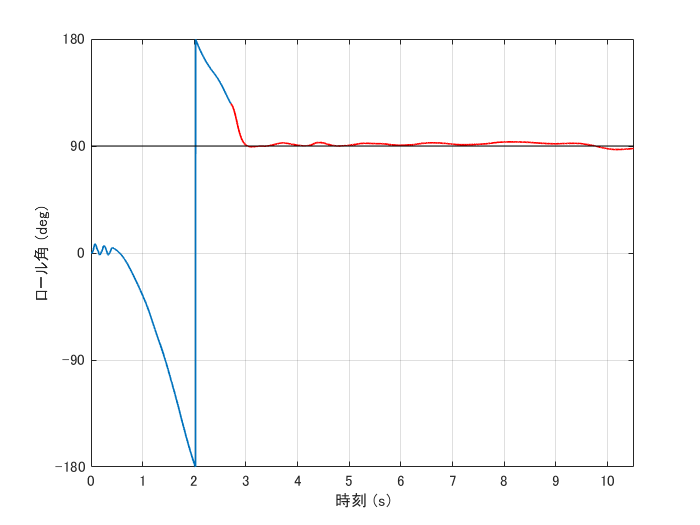
\includegraphics[width=0.8\linewidth]{pic_avi/ロール角.png}
	\caption{ロール角の時間変化}
	\label{fig:ロール角}
\end{figure}
図\ref{fig:動翼角度}に離床から制御終了までの動翼角度の時間変化を青色で示す。また、目標動翼角度の時間変化を黒色で示す。
動翼角度が目標値に高い精度で追従していることが分かる。図\ref{fig:動翼角度_切り取り}に離床後2.7秒から2.9秒までを抜き出したグラフを示す。
動翼角度が目標値にわずかに遅れて追従していることが分かる。離床後約2.76秒から約2.79秒までの間、目標値が-15度で一定値なのに対して動翼角度が約14.74度で停止しており、誤差がある。
これは、空力により動翼の軸まわりにはたらくモーメントの影響だと考えられる。
エンジン燃焼終了から間もないため対気速度が大きく、動翼角度の絶対値も大きいため、モーメントが大きい状況であり、誤差が大きくなったと考えられる。
\begin{figure}[H]
	\centering
	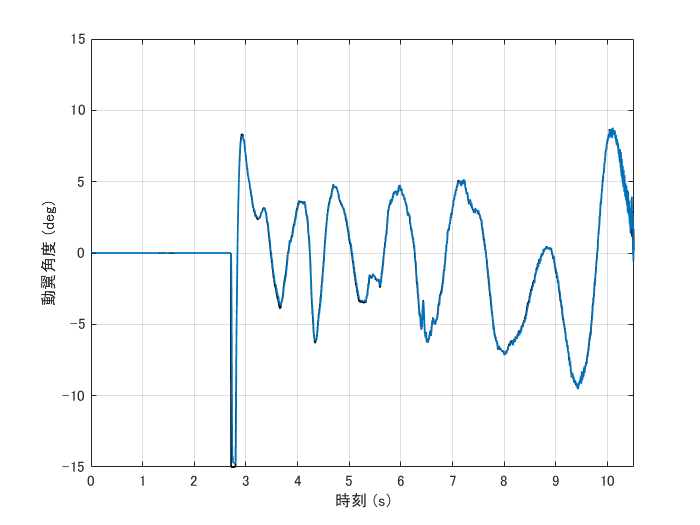
\includegraphics[width=0.8\linewidth]{pic_avi/動翼角度.png}
	\caption{動翼角度と目標動翼角度の時間変化}
	\label{fig:動翼角度}
\end{figure}
\begin{figure}[H]
	\centering
	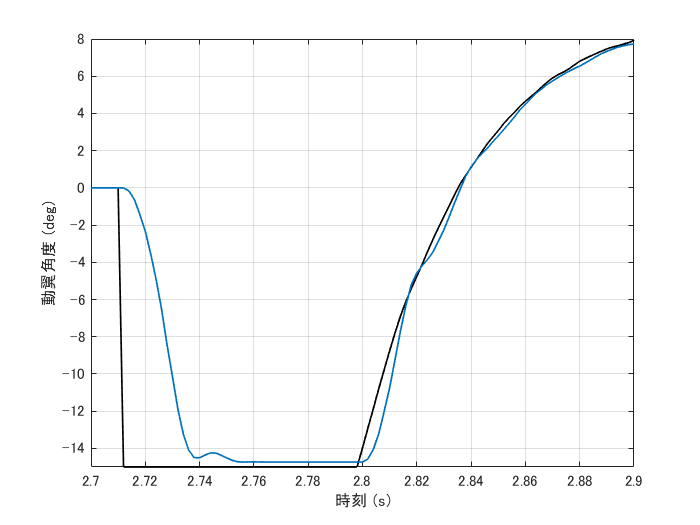
\includegraphics[width=0.8\linewidth]{pic_avi/動翼角度_切り取り.png}
	\caption{離床後2.7秒から2.9秒までの動翼角度と目標動翼角度の時間変化}
	\label{fig:動翼角度_切り取り}
\end{figure}
\end{document}